\ifdefined\DIPLOMA
    \subsubsection{Описание объекта управления}
    \label{sec_controlled_object_desc}
\else
    \subsection{Описание объекта управления}
\fi

Проектируемый привод установлен на малом спутнике Земли и представляет собой
исполнительный элемент системы дистанционного зондирования Земли (далее~-- ДЗЗ).
Объектом управления является специальная камера (рис. \ref{control_object_general_view}),
предназначенная для создания снимком поверхности Земли высокой четкости,
оборудована двумя звёздными датчиками для ориентации в пространстве и
находящаяся внутри корпуса экранно~--~вакуумной теплоизоляции (далее~-- ЭВТИ).

\begin{figure}[ht!]
    \centering
    \begin{minipage}{0.45\textwidth}
        \centering
        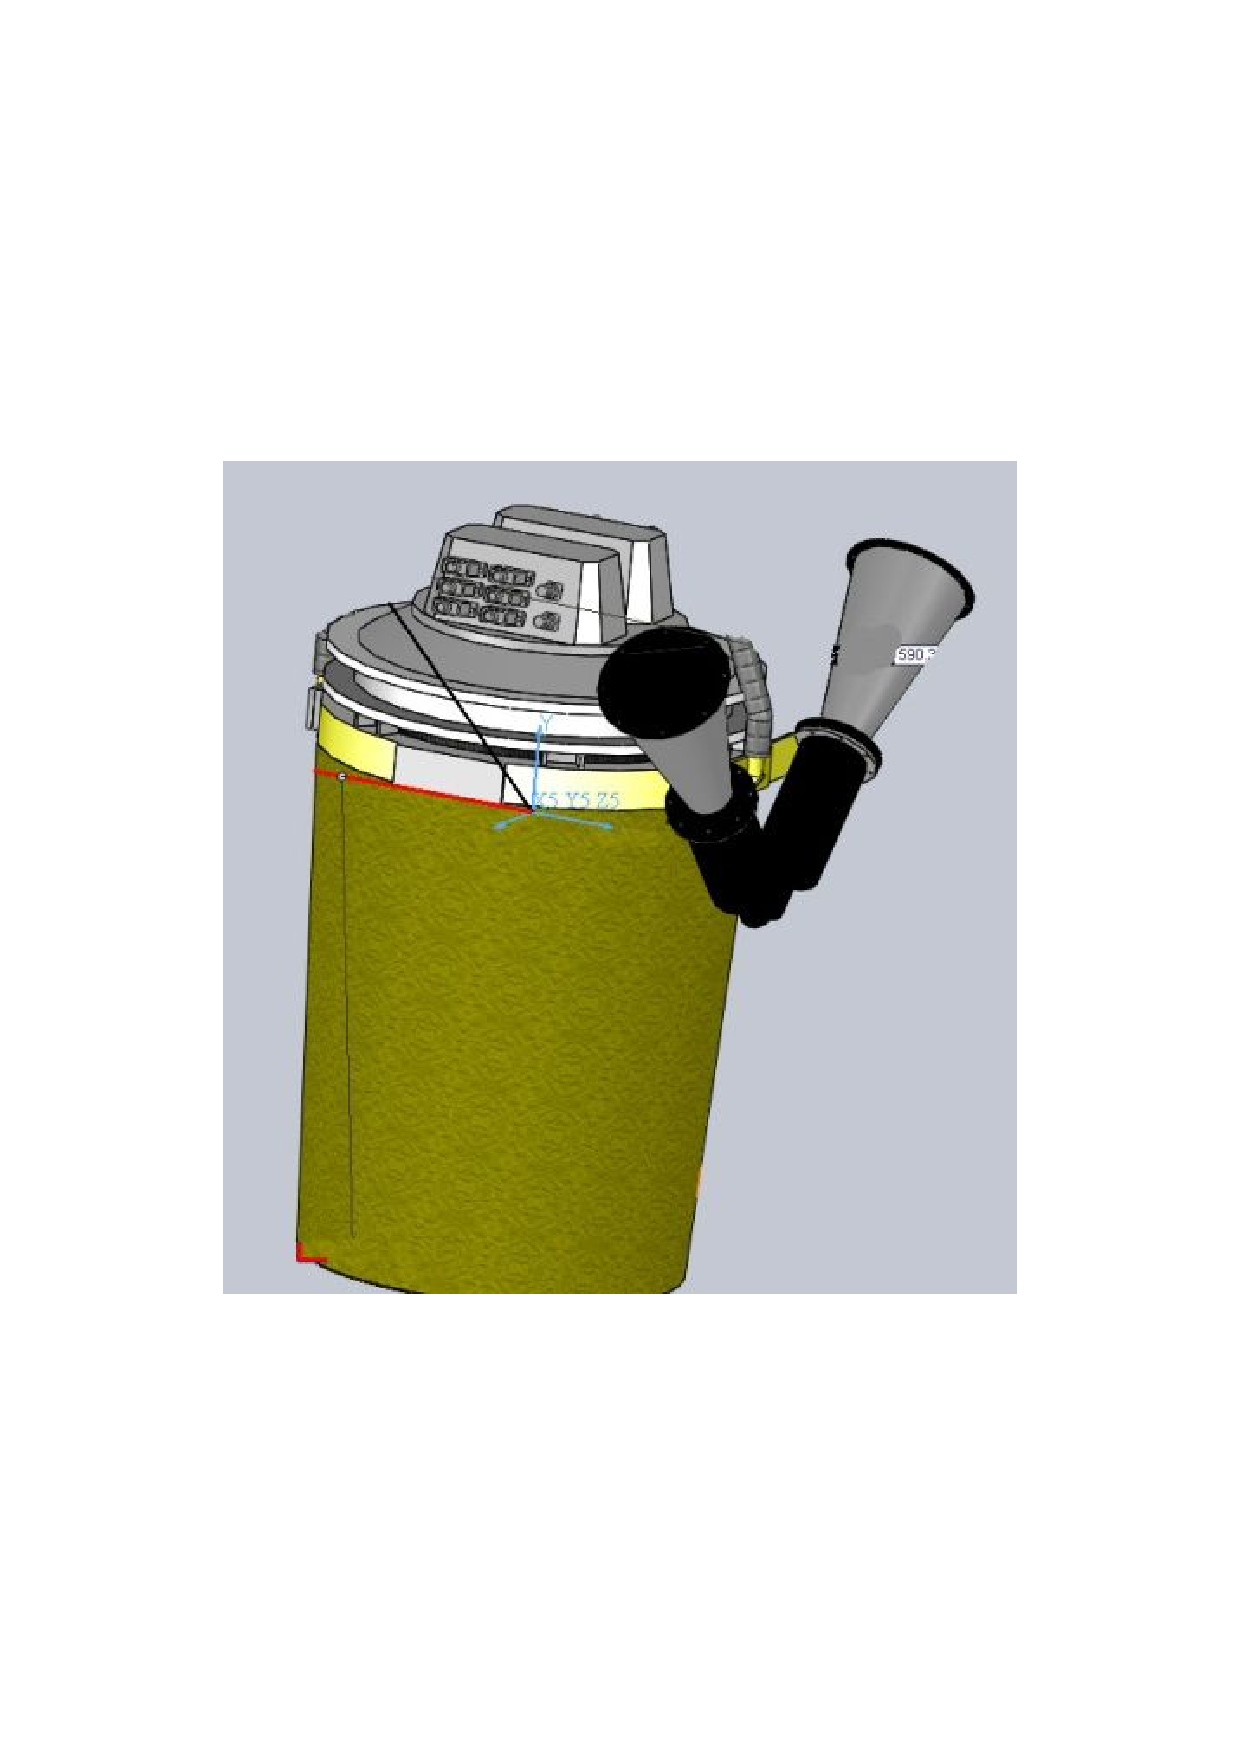
\includegraphics[width=0.5\linewidth, keepaspectratio]
                        {./src/pictures/sattelite_3d_images/control_object_view_1}
        \label{control_object_view_1}
    \end{minipage}~
    \begin{minipage}{0.45\textwidth}
        \centering
        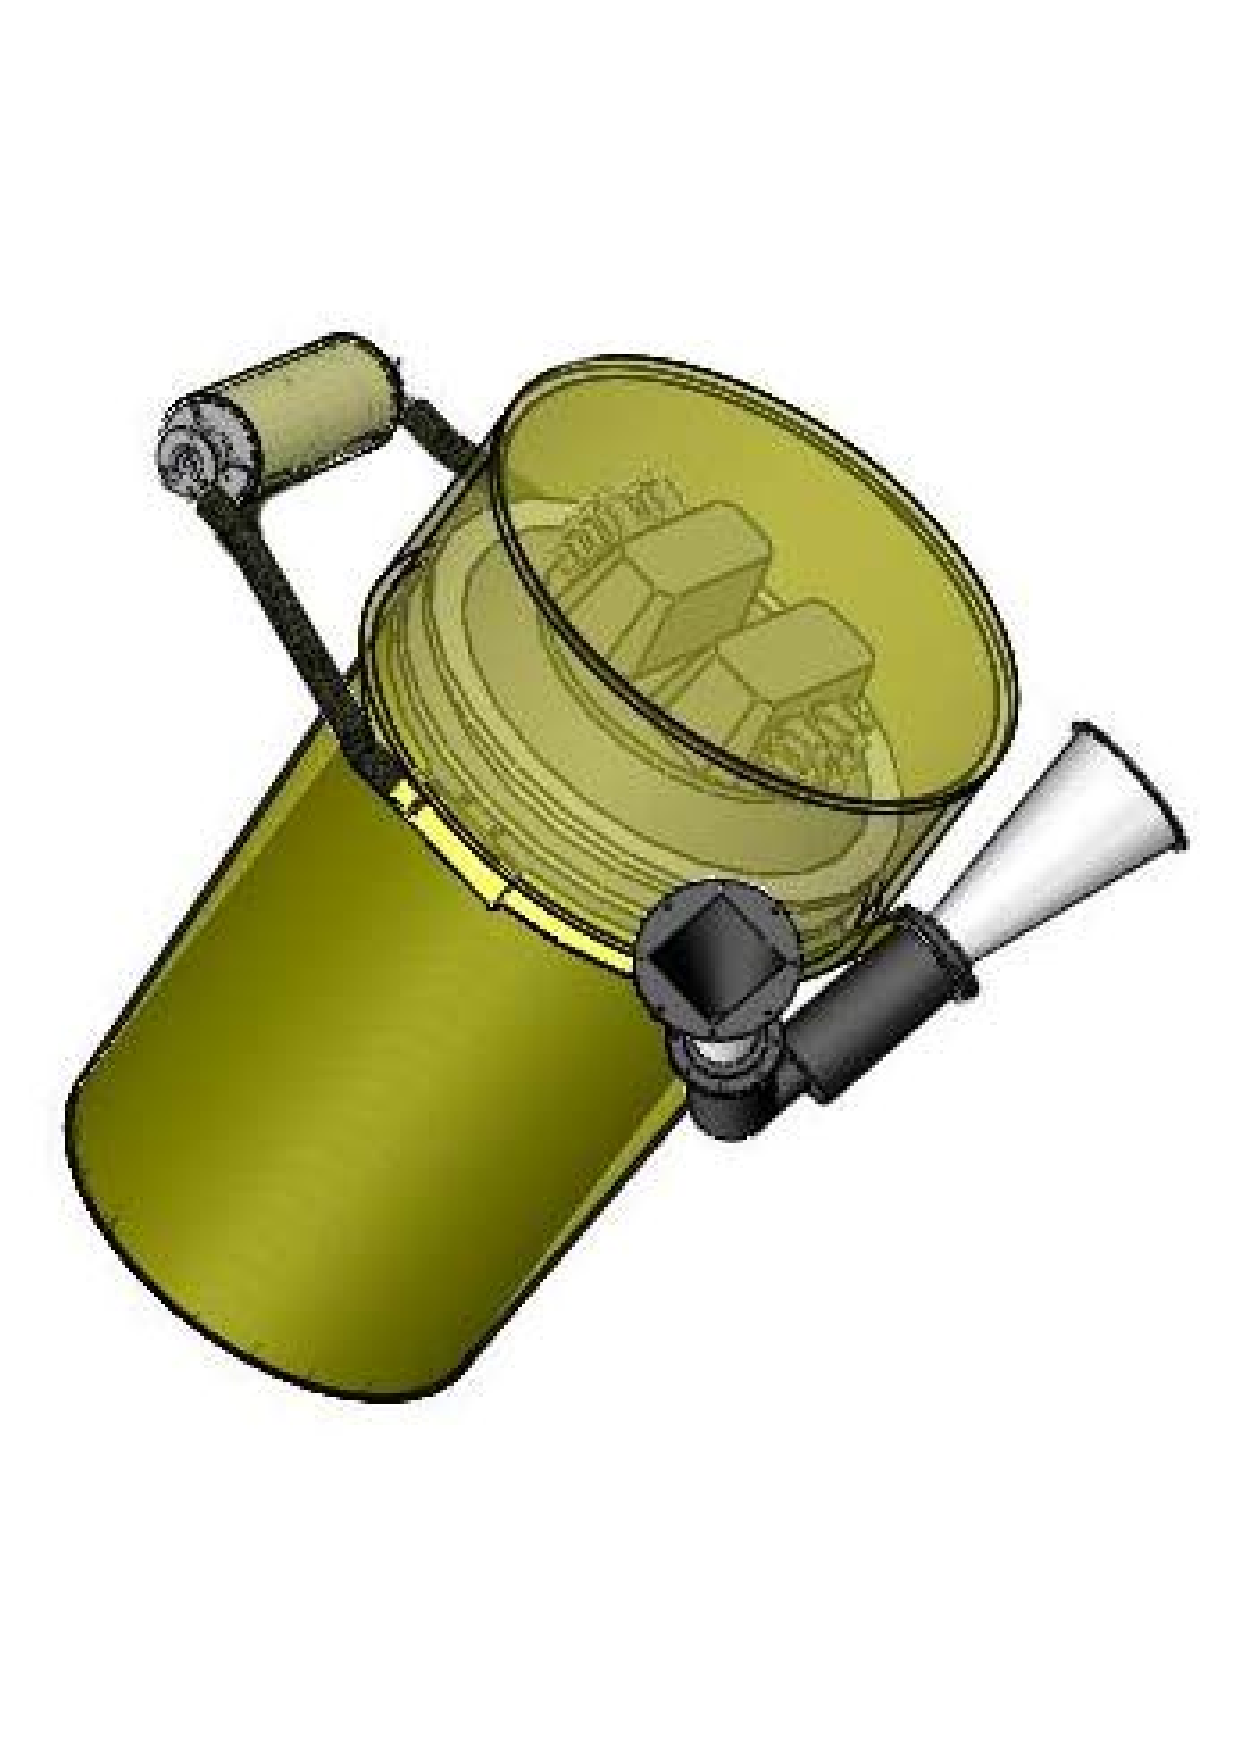
\includegraphics[width=0.5\linewidth, keepaspectratio]
                        {./src/pictures/sattelite_3d_images/control_object_view_2}
        \label{control_object_view_2}
    \end{minipage}

    \caption{Общий вид объекта управления}
    \label{control_object_general_view}
\end{figure}

\begin{table}[ht!]
    \centering
    \begin{tabu} spread \textwidth {X[-1,c,m]|X[l,m]}                                                   \hline
        Изображение & Описание                                                                          \\ \hline
        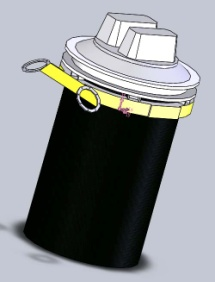
\includegraphics[width=0.1\textwidth, keepaspectratio]
                        {./src/pictures/sattelite_3d_images/camera}
        &
        \textbf{Камера ДЗЗ:}                                                                            \newline
        Момент инерции вокруг продольной оси: $1.22 ~\textit{кг} \cdot \textit{м}^{2}$                  \newline
        Момент инерции вокруг каждой из двух поперечных  осей: $2.17 ~\textit{кг} \cdot \textit{м}^{2}$ \newline
        Масса: $49.84 ~\textit{кг}$                                                                     \\ \hline

        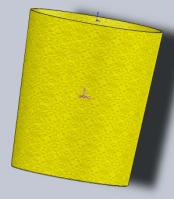
\includegraphics[width=0.1\textwidth, keepaspectratio]
                        {./src/pictures/sattelite_3d_images/bottom_shell_part}
        &
        \textbf{Нижняя часть ЭВТИ:}                                                                     \newline
        Момент инерции вокруг продольной оси: $0.18 ~\textit{кг} \cdot \textit{м}^{2}$                  \newline
        Момент инерции вокруг каждой из двух поперечных  осей: $0.18 ~\textit{кг} \cdot \textit{м}^{2}$ \newline
        Масса: $4.37 ~\textit{кг}$                                                                      \newline
        Продольная длина: $0.5 ~\textit{м}$                                                             \\ \hline

        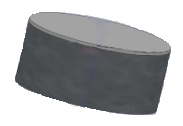
\includegraphics[width=0.1\textwidth, keepaspectratio]
                        {./src/pictures/sattelite_3d_images/top_shell_part}
        &
        \textbf{Верхняя часть ЭВТИ:}                                                                    \newline
        Момент инерции вокруг продольной оси: $0.07 ~\textit{кг} \cdot \textit{м}^{2}$                  \newline
        Момент инерции вокруг каждой из двух поперечных  осей: $0.04 ~\textit{кг} \cdot \textit{м}^{2}$ \newline
        Масса: $1.53 ~\textit{кг}$                                                                      \newline
        Продольная длина: $0.25 ~\textit{м}$                                                            \\ \hline

        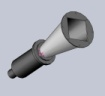
\includegraphics[width=0.1\textwidth, keepaspectratio]
                    {./src/pictures/sattelite_3d_images/star_sensor}
        &
        \textbf{Звездный датчик (2 шт.):}                                                               \newline
        Момент инерции вокруг продольной оси: $0.0 ~\textit{кг} \cdot \textit{м}^{2}$                   \newline
        Момент инерции вокруг каждой из двух поперечных  осей: $0.02 ~\textit{кг} \cdot \textit{м}^{2}$ \newline
        Масса: $2.08 ~\textit{кг}$                                                                      \\ \hline

        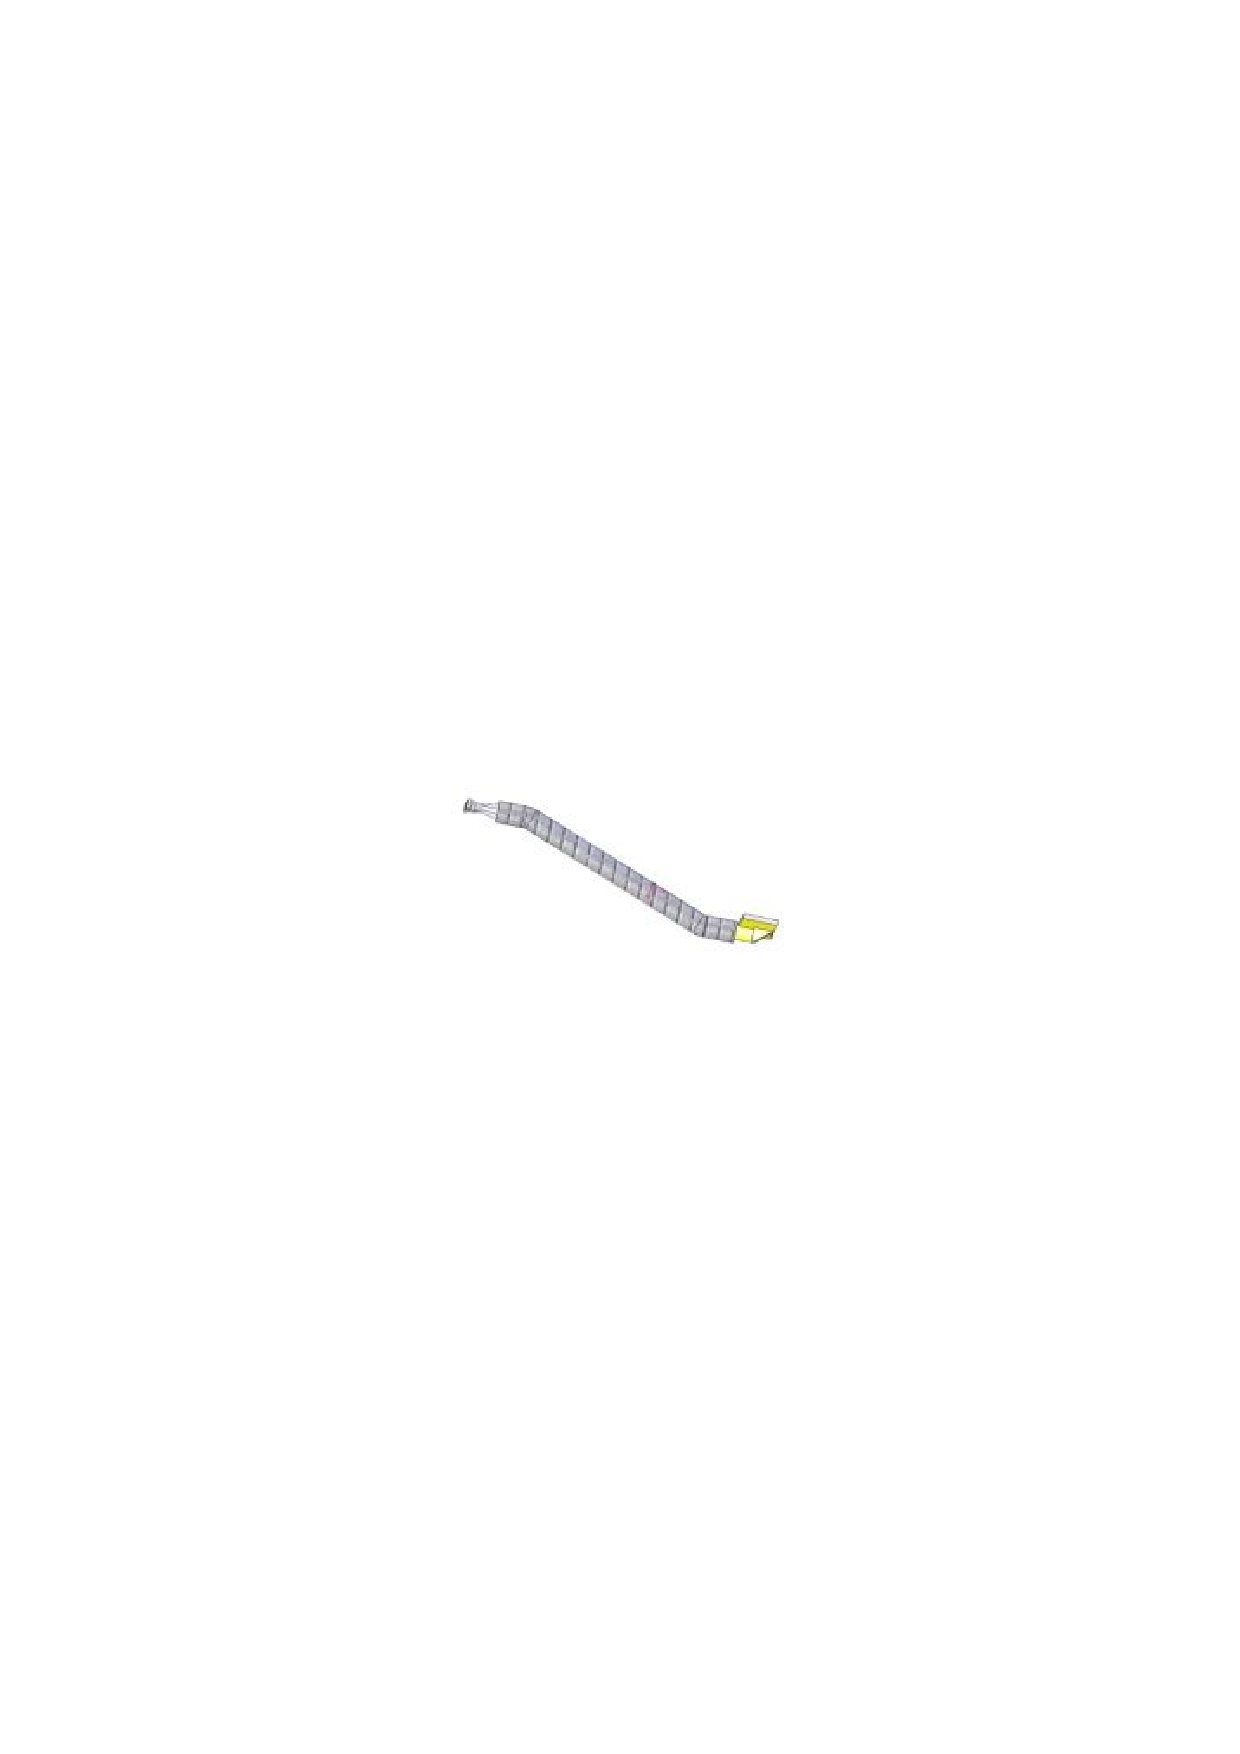
\includegraphics[width=0.1\textwidth, keepaspectratio]
                    {./src/pictures/sattelite_3d_images/sleeve}
        &
        \textbf{Рукав (2 шт.):}                                                                         \newline
        Момент инерции вокруг продольной оси: $0.0 ~\textit{кг} \cdot \textit{м}^{2}$                   \newline
        Момент инерции вокруг каждой из двух поперечных  осей: $0.02 ~\textit{кг} \cdot \textit{м}^{2}$ \newline
        Масса: $0.3 ~\textit{кг}$                                                                       \\ \hline
    \end{tabu}

    \caption{Составные элементы объекта управления}
\end{table}

Общая масса камеры и ее навесных элементов: $60.5 ~\textit{кг}$. С учетом запаса, выберем
массу объекта управления манипулятора: $80 ~\textit{кг}$.
Расстояние от оси привода до центра масс камеры: $400 ~\textit{мм}$ (с учетом запаса
на более габаритную камеру и запаса на ускорение камеры);
Собственный момент инерции объекта управления вокруг оси, параллельной оси привода:
$ J_{oy} = 2.84 ~\textit{кг}~\cdot~\textit{м}^2 $

Момент инерции объекта управления относительно оси привода:
$ J = 15.7 ~\textit{кг}~\cdot~\textit{м}^2 $

\textit{Примечание:} полученная величина момента инерции объекта управления относительно
оси привода 2 соответствует величине, вычисленной с помощью программы Autodesk Inventor.
